%% LyX 2.3.4.2 created this file.  For more info, see http://www.lyx.org/.
%% Do not edit unless you really know what you are doing.
\documentclass[letterpaper,english,reprint,superscriptaddress,groupedaddress,pra,aps]{revtex4-1}
\usepackage[T1]{fontenc}
\usepackage[latin9]{inputenc}
\setcounter{secnumdepth}{3}
\usepackage{color}
\usepackage{babel}
\usepackage{mathtools}
\usepackage{amsmath}
\usepackage{amssymb}
\usepackage{graphicx}
\usepackage[unicode=true,pdfusetitle,
 bookmarks=true,bookmarksnumbered=false,bookmarksopen=false,
 breaklinks=false,pdfborder={0 0 1},backref=false,colorlinks=false]
 {hyperref}
\hypersetup{
 colorlinks,linkcolor=red,anchorcolor=black,citecolor=blue}

\makeatletter

%%%%%%%%%%%%%%%%%%%%%%%%%%%%%% LyX specific LaTeX commands.
\special{papersize=\the\paperwidth,\the\paperheight}


\makeatother

\begin{document}
\preprint{APS/123-QED}
\title{Investigating the quench dynamics of the edge states of a spin-orbital
coupling system using a trapped ion}
\thanks{A footnote to the article title}
\affiliation{CAS Key Laboratory of Quantum Information, University of Science and
Technology of China, Hefei, 230026, People Republic of China.and CAS
Center For Excellence in Quantum Information and Quantum Physics,University
of Science and Technology of China, Hefei, 230026, People Republic
of China. }
\collaboration{MUSO Collaboration }
\date{\today}
\begin{abstract}
The quantum walk (QW), as the quantum analogue of classical random walk, provides feasible platform to study topological phenomenon and non-equilibrium dynamics. Here, we propose a novel scheme to realize the quantum walk with a single trapped ion where the phonon number space provides the natural boundary of the QW. In this scheme, the natural boundary offer the unique opportunity to investigate the dynmaics of the edge states of the corresponding topological systems. Paricularly, the quench dynamics of the edge state are  extensively studied by tuning the local vacuum operator. Our proposal offer a new approach to explore the character of the edge states of the topological systems and the difference of the quench dynamics of the edge states also offer the way to determine the boundary of differnt phases of the system.
\begin{description}
\item [{Usage}] Secondary publications and information retrieval purposes.
\item [{PACS~numbers}] May be entered using the environment \textsf{PACS~numbers}.
\item [{Structure}] You may use the \texttt{Description} environment to
structure your abstract.
\end{description}
\end{abstract}
\pacs{33.15.Ta}
\keywords{Suggested keywords}

\maketitle


\section{Introduction}

The topological matter has been studied extensively recently in different
platform \citep{laughlin1983anomalous,wang2009observation,hasan2010colloquium,qi2011topological,stuhl2015visualizing}.
One of the interesting feature is that the topological matter is protected
by topology against local perturbations, such as, the quantization
of Hall conduct is robust under impurity \citep{von1986quantized,nagaosa2010anomalous,stormer1999fractional};
another unique character of the topology matter is the appearance
of the edge state at the boundary of the sample \citep{jackiw1976solitons,su1979solitons}.
The bulk topological invariants and the number of the edge states
can be connected by the bulk-edge correspondence \citep{wen1992theory,hasan2010colloquium}.

Though the equilibrium properties have been widely explored, the non-equilibrium
dynamics of topological system is still under investigation \citep{heyl2018dynamical}(Dynamical
quantum phase transition \citep{heyl2017dynamical}, Dynamical chern
number, linking number \citep{PhysRevLett.118.185701,flaschner2018observation,tarnowski2019measuring}).
The quench process is the typical non-equilibrium process which have
been studied in different topological systems. On one hand, the bulk
topological invariants, such as Chern number, is known to be unchanged
under unitary dynamics \citep{d2015dynamical,caio2015quantum} and
they are unchanged during the quench processes. However, the non-unitary
processes, such as the dissipation or decoherence process, will change
the bulk topological invariants during quench process \citep{aidelsburger2011experimental,aidelsburger2013realization,atala2014observation}.
Since the bulk-edge correspondence is only valid for the equilibrium
situation\citep{d2015dynamical,caio2015quantum,wilson2016remnant,hu2016dynamical},
the dynamics of the edge states in the boundary of the topological
system is still elusive \citep{wang2019experimental,yi2019observing},
for example, Ref. \citep{caio2015quantum} studies quenches between
topological and non-topological phases in Haldane model, while observing
presence or absence of edge modes; Ref. \citep{hu2016dynamical}.
To investigate the dynamics of the edge states have attracted a lot
of attention \citep{d2015dynamical}. In addition, how to experimentally
observe the dynamics of the edge state is still an open question. 

The quantum walk (QW), which can be used to construct universal quantum
computation\citep{childs2009universal,childs2013universal}, has been
shown to be a powerful platform to study the equilibrium and non-equilibrium
topological properties of spin-orbital systems \citep{PhysRevA.82.033429,Kitagawa2012,asboth2012symmetries,asboth2013bulk,asboth2014chiral,obuse2015unveiling,barkhofen2017measuring,cardano2016statistical,flurin2017observing,mochizuki2016explicit,xiao2017observation,schreiber2010photons,crespi2013anderson}.
Particularly, it has been used to observe the bound states \citep{kitagawa2012observation,chen2018observation,nitsche2019eigenvalue}.
Different QWs have been experimentally realized in different experiment
platform, such as photonics\citep{kitagawa2012observation,schreiber2010photons,broome2010discrete,chen2018observation,xu2018measuringd,xu2018measuringw},
neutral atoms \citep{karski2009quantum,mugel2016topological}, superconductor
\citep{flurin2017observing,yan2019strongly} and trapped ion \citep{xue2009quantum,zahringer2010realization}. 

The trapped ions system, which can be accurately controlled and manipulated
\citep{leibfried2003quantum,blatt2012quantum}, is one of the most
idea platform for investigating quantum information processing and
no-equilibrium dynamics of many-body system \citep{eisert2015quantum,zhang2017observationm,zhang2017observationt}.
Particularly, QW has been realized in one or two trapped $^{40}\text{Ca}^{+}$
ions by the phase space operation \citep{xue2009quantum,zahringer2010realization}.
Here, we proposed to encode QW on the Fock space of the phonon, which
is similar to the Ref. \citep{oka2005breakdown} and the zero-number
phonon state (the vacuum state) acts as the natural boundary of the
QW. With carefully designed the laser sequences, the dynamics of the
edge state can be experimentally investigated. We carefully analyze
the quench dynamics of the edge state by tuning different parameters
in this system.

\section{THEORETICAL BACKGROUND\label{sec:2}}

One dimensional discrete QW is quantum version of the classical random
walk. The walker is described by two internal states (denoted by$\left|\uparrow\right\rangle ,\left|\downarrow\right\rangle $
and the position state (labeled as $\left|x\right\rangle $), and
the internal state and the position state can be coupled through the
coin operation $R(\theta,x)$ ($\theta$ is the control parameter
and it may dependent on the position of the walker $x$). We focus
on the split-step quantum walk (SSQW) and its one-step floquet operator
$U(\theta_{1},\theta_{2})$ is defined as: 
\begin{eqnarray}
U(\theta_{1},\theta_{2}) & = & S_{+}R(\theta_{2})S_{-}R(\theta_{1})\label{eq:1}
\end{eqnarray}
where $S_{\pm}$ is defined as $\sum|i\pm1\rangle\langle i|\otimes|\uparrow\rangle\left\langle \uparrow\left|+1\otimes\right|\downarrow\right\rangle \langle\downarrow|$
and $R(\theta)=\sum_{i}|i\rangle\langle i|\otimes\mathrm{e}^{-\mathrm{i}\sigma_{y}\theta/2}$
(the coin operator is independent of the position $x$). The quantum
state of the SSQW can be obtained by: $|\Psi\rangle_{n}=U^{n}(\theta_{1},\theta_{2})|\Psi\rangle_{0}$
where $|\Psi\rangle_{0}$ is the initial state of the evolution (generally,
we begin the evolution of the system with a product state). The effective
Hamiltonian of this periodical system can be derived from $U(\theta_{1},\theta_{2})=e^{-iH_{\mathrm{eff}}}$,
and $H_{\text{eff}}=\int_{k}E(k)n(k)\cdot\sigma\otimes|k\rangle\langle k|$
in momentum space, where the dispersion relation and Bloch vector:

\begin{align}
\cos E(k) & =\cos\left(\theta_{2}/2\right)\cos\left(\theta_{1}/2\right)\cos k-\sin\left(\theta_{1}/2\right)\sin\left(\theta_{2}/2\right)\nonumber \\
n_{x}(k)= & \frac{\cos\left(\theta_{2}/2\right)\sin\left(\theta_{1}/2\right)\sin k}{\sin E(k)}\nonumber \\
n_{y}(k)= & \frac{\sin\left(\theta_{2}/2\right)\cos\left(\theta_{1}/2\right)+\cos\left(\theta_{2}/2\right)\sin\left(\theta_{1}/2\right)\cos k}{\sin E(k)}\nonumber \\
n_{z}(k)= & -\frac{\cos\left(\theta_{2}/2\right)\cos\left(\theta_{1}/2\right)\sin k}{\sin E(k)},
\end{align}

with $\sigma=(\sigma_{x},\sigma_{y},\sigma_{z})$. To determine the
phase diagram of the QW, two different time frames which are defined
by: 
\begin{eqnarray}
U_{1}(\theta_{1},\theta_{2})=R\left(\theta_{1}/2\right)S_{+}R\left(\theta_{2}\right)S_{-}R\left(\theta_{1}/2\right),\nonumber \\
U_{2}(\theta_{1},\theta_{2})=R\left(\theta_{2}/2\right)S_{-}R(\theta_{1})S_{+}R\left(\theta_{2}/2\right).\label{eq:2}
\end{eqnarray}
should be considered. These two time frames have chiral symmetry and
the whole phase diagram can be described by a pair of $\mathbb{Z}_{2}\times\mathbb{Z}_{2}$
topological invariants \citep{asboth2013bulk}:
\begin{eqnarray}
\nu_{0}=\frac{1}{2}+\frac{1}{2}(\nu^{\prime}+\nu^{\prime\prime}),\nonumber \\
\nu_{\pi}=\frac{1}{2}+\frac{1}{2}(\nu^{\prime}-\nu^{\prime\prime}),\label{eq:3}
\end{eqnarray}
 where $\nu^{\prime}$ is the winding of the eigen-state in the first
time frame and $\nu^{\prime\prime}$ is the winding in the second
time frame (see Fig. \ref{fig:1}).

\begin{figure*}
\mbox{%
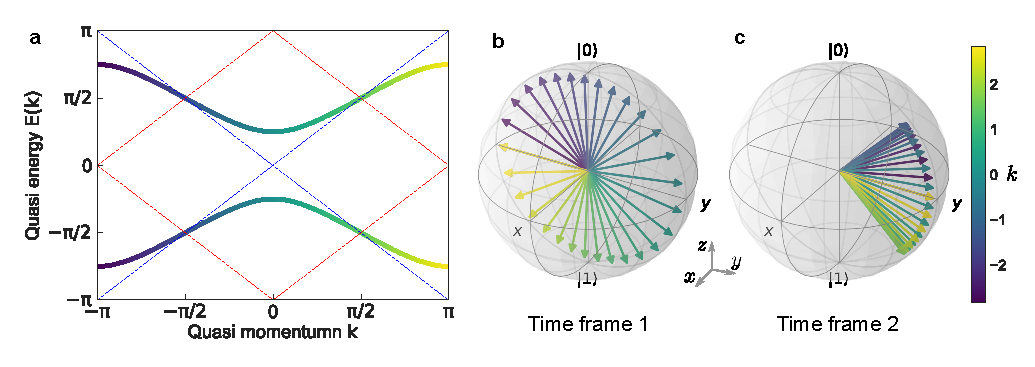
\includegraphics[width=17.5cm]{Figure/fig_1}%
}\caption{\label{fig:1} Split-step quantum walk with the parameters $\theta_{1}=\frac{\pi}{2}$,
$\theta_{2}=0$. a shows the dispersion relationship which is independent
of the time frame; the blue and red dash lines represent the cases
which the energy gap close at the quasi-energy 0 and $\pi$and character
the phase transition points. b and c correspond to the two time frames
with chiral symmetry to obtain the $\mathbb{Z}_{2}\times\mathbb{Z}_{2}$
topological invariants. In the cases, $\nu^{\prime}=1$, $\nu^{\prime\prime}=0$
thus based on Eq. \ref{eq:3}, $\nu_{0}=1$, $\nu_{\pi}=0$.}
\end{figure*}

Due to the topological character of the different phases in the QW,
when crossing one phase to another topological phase in the real space,
there is a bound state appear at the boundary of these two phases.
In one dimensional QW, the bound state can be formed with inhomogeneous
rotations in space between distinct regions and it has been observed
\citep{kitagawa2012observation}. The different topological invariants
in the two phases guarantee the robust of the bound state. Especially,
the vacuum can be viewed as a special phase and the bound state can
appear at the boundary of a semi-finite QW system (see Sup. \ref{sec:A}
for a simple model with analytical eigen-state results).

In order to investigate the dynamics of the bound state between the
quench of the system, we first evolved the system with initial effective
hamiltonian $H_{\text{eff}}(\theta_{1}^{i},\theta_{2}^{i})$ to form
a stable bound state at the boundary. Then, suddenly (or slowly) changing
the effective Hamiltonian of the system to the final Hamiltonian $H_{\text{eff}}(\theta_{1}^{f},\theta_{2}^{f})$
(or slowly change the parameter $(\theta_{1}^{i},\theta_{2}^{i})$
to $(\theta_{1}^{f},\theta_{2}^{f})$ along some path ) and observe
the dynamics of the bound state. The dynamics is strongly dependent
of the quench parameter and the local manipulation of the boundary
site. \textcolor{red}{Is it possible to change the bond state by local
operator?->twisted boundary condition, the boundary of the material
define the bulk topology.}

\section{EXPERIMENT PROPOSAL\label{sec:3}}

\begin{figure*}
\mbox{%
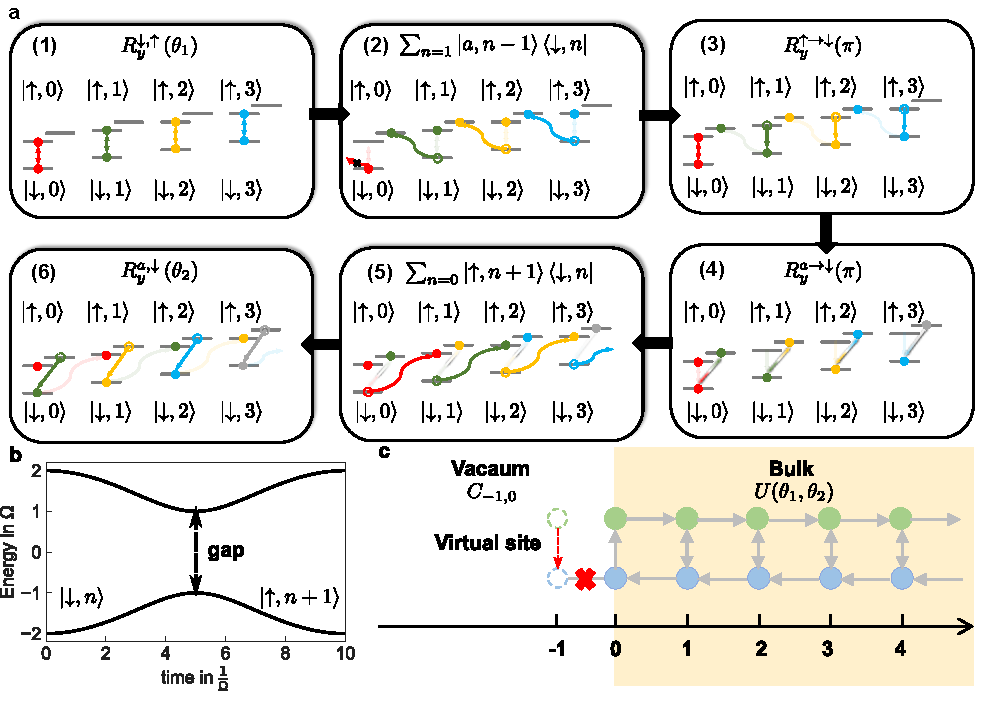
\includegraphics[width=17.5cm]{Figure/fig_2}%
}\caption{\label{fig:2} a. Pulse sequences to realize QW with boundary. $\left|\uparrow,n\right\rangle $
and $\left|\downarrow,n\right\rangle $ represent for $\left|n\right\rangle \otimes\left|\uparrow\right\rangle $
and $\left|n\right\rangle \otimes\left|\downarrow\right\rangle $
with $\left|F=1,m_{F}=0\right\rangle \protect\coloneqq\left|\uparrow\right\rangle $
and $\left|F=0,m_{F}=1\right\rangle \protect\coloneqq\left|\downarrow\right\rangle $
of $^{2}S_{1/2}$ manifold, $|n\rangle$ for the state of the phonon
with $n$ phonon. Auxiliary level $\left|a\right\rangle $ works for
temporal state shelving and it has no occupation after the whole operations.
Six steps are required for $U(\theta_{1},\theta_{2})$ along the black
arrow direction. Step one and four are rotation operations which mix
spin and other steps are for spin-dependent shifting. Phonon number
deduces one in step two while blocked at $\left|\downarrow,0\right\rangle $
and then flips to $\left|\uparrow,0\right\rangle $ in step three
so it simulates the spin flipping operation at boundary. Adiabatic
processes in step two and five fix the problem of phonon shifting
simultaneously, works as an adiabatically $\pi$flipping between upper
and lower state. b. Eigen-energy of modulated Jaynes-Cummings model
$H(t)$ in subspace $\left|\downarrow,n\right\rangle \leftrightarrow\left|\uparrow,n+1\right\rangle $
(in the unit of $\Omega$). Rabi frequency $\Omega$ equals to detuning
$\delta$, while total transition time sets to be $\frac{10}{\Omega}$.
The adiabatic condition is satisfied when the evolution is much slower
the time scale set by the energy gap, then adiabatically transform
state from $\left|\downarrow,n\right\rangle $ to $\left|\uparrow,n+1\right\rangle $
for all $n$. c. Bulk togological invariant is defined with boundary
condition. With introducing virtual site at $n=-1$ lattice, we can
define the boundary ``cut link'' operator $C_{-1,0}$ (thus vacuum)
then bulk phase with different $(\theta_{1},\theta_{2})$.}
\end{figure*}

Trapped ion system have been proved as a powerful platform for quantum
simulation. Here, we propose a way to realize the QW with boundary
by a single $^{171}\text{Yb}^{+}$ ion in a three-dimensional Harmonic
trap. In this system, the two level internal state of the QW (we call
spin) is encoded in the $\left|F=1,m_{F}=0\right\rangle \coloneqq\left|\uparrow\right\rangle $
and $\left|F=0,m_{F}=1\right\rangle \coloneqq\left|\downarrow\right\rangle $
of $^{2}S_{1/2}$ hyperfine manifold of ion $^{171}\text{Yb}^{+}$
with splitting $\omega_{\text{Hpf}}=2\pi\times12.6\text{\text{GHz}}$;
and the lattice sites of the QW are encode in the number of the phonons
where the zero phonon state provide the natural boundary of the QW.
To realize the QW, we need to implement two different basic operators
$R(\theta)$ and $S_{\pm}$. The rotation operator $R(\theta)$ is
easy to realize by manipulate the hyperfine state ($|\uparrow\rangle$
and $|\downarrow\rangle$) by microwave or by Stimulate-Raman-Process.
To implement the operator $S_{\pm}$ in the phonon space needs more
work and is a bit complicated, where the auxiliary Zeeman energy level
$\left|F=1,m_{F}=1\right\rangle \coloneqq\left|a\right\rangle $ will
introduced to provide temporary shelving states. 

Generally, the interaction between the internal state ($\left|\downarrow\right\rangle $
and $\left|\uparrow\right\rangle $) and the phonons with frequency
$\omega_{\text{phon}}$ can be induced by a pair of proper selected
stimulated Raman beams with frequency $\omega_{\text{Raman1}}$ and
$\omega_{\text{Raman2}}$ , and the interaction can be described by
the effective two level Jaynes-Cummings Hamiltonian $H_{\text{JC}}=\frac{\Omega}{2}a\sigma_{+}e^{i\delta t}+\text{h.c.}$
under the rotation wave approximation (RWA), where $\Omega$ is the
effective Rabi frequency, $\omega_{\text{Raman1}}-\omega_{\text{Raman2}}=\omega_{\text{Hpf}}\pm\omega_{\text{phon}}+\delta$
(red (blue) sideband corresponded $-$($+$) and phonon frequency
$\omega_{\text{phon}}$) , $a^{+}=\sum_{n=0}\sqrt{n+1}\left|n+1\right\rangle \left\langle n\right|$
($a=\sum_{n=1}\sqrt{n}\left|n-1\right\rangle \left\langle n\right|$)
is the creation (annihilation) operation of phonon, $\sigma_{+}(\sigma_{-})$
is the flipping operation $\left|\uparrow\right\rangle \left\langle \downarrow\right|$
($\left|\downarrow\right\rangle \left\langle \uparrow\right|$) of
spin. With this integration, the number of the phonons can be manipulated:
the red sideband beam gives the transition of $\left|n\right\rangle \otimes\left|\downarrow\right\rangle \leftrightarrow\left|n-1\right\rangle \otimes\left|\uparrow\right\rangle $
with Rabi frequency $\Omega_{n,n-1}=\sqrt{n}\Omega$ and the blue
sideband gives the transition of $|n\rangle\otimes|\downarrow\rangle\leftrightarrow|n+1\rangle\otimes|\uparrow\rangle$
with Rabi frequency $\Omega_{n,n+1}=\sqrt{n+1}\Omega$, where $\left|n\right\rangle $
is the state of the phonon with $n$ phonon. The controlled hopping
between the state with different number of phonons is almost the same
as the operator $S_{\pm}$ besides the Rabi frequency is dependent
of the number of the phonon (lattice site of the QW) . The phonon
number dependence introduces additional difficulty, as a result, to
implement the hopping operators $S_{\pm}$ homogeneously is the main
obstacle to realize the QW in this system. 

Actually, the hopping operator $S_{\pm}$ indeed can be realized by
some adiabatic processes (called Stimulated Raman Adiabatic Passage
(STIRAP) ) which has already been used to cool the motional state
in Ref. \citep{king1998cooling,wunderlich2007robust} and solve the
imhomogenious hopping \citep{um2016phonon}. According to the adiabatic
theorem \citep{simon1983holonomy}, when Hamiltonian of the system
changes slowly enough \citep{wunderlich2007robust}, the system will
keep on the same eigen-state of the Hamiltonian for all the time if
its initial state is a eigen-state of the initial Hamiltonian. In
our current experimental setup, we can set $\Omega(t)=\Omega\sin(\frac{\pi t}{\tau})$
and $\delta(t)=\delta\cos(\frac{\pi t}{\tau})$ ($\tau$ is the total
operation time) in the Hamiltonian $H_{\text{\text{JC}}}$ to construct
the time dependent Hamiltonian $H(t)$ in the adiabatic process. The
initial state $\left|n\right\rangle \otimes\left|\downarrow\right\rangle $
is the lower eigen-state of the two-band Hamiltonian $H(0)$, when
the parameter satisfies the adiabatic condition $\frac{d\theta(t)}{dt}\ll\text{gap}$
($\tan(\theta(t))=\frac{\Omega(t)}{\delta(t)}$ is the angle on the
Bloch sphere during the evolution). The system will keep evolving
along the lower band of $H(t)$ and stay at the corresponding eigen-state
of $H(\tau)$. The adiabatic process is not dependent on the number
of the phonon if the order of the eigen-states is given, see Fig.
\eqref{fig:2}b for eigen-energy with given parameters during the
whole process. \textcolor{red}{Give a level graph of H(t) to show
the connection of the corresponding eigen-state} In order to speed
up adiabatic process, further methods to suppress the non-adiabatic
excitation \citep{um2016phonon} and to reshape the waveform for shortcut
Raman passage has been proposed and realized in experiment \citep{du2016experimental}. 

Therefore, based on the STIRAP method, the key operators $R(\theta)$
and $S_{\pm}$ for the QW can be realized in a trapped ion and the
whole QW evolution $U(\theta_{1},\theta_{2})$ can be realized by
the following six steps. For convenience, we define $\Delta\omega=\omega_{\text{Raman1}}-\omega_{\text{Raman2}}$
and Zeeman splitting under magnetic field $\omega_{\text{Zm}}$:
\begin{enumerate}
\item Apply rotation $R_{y}(\theta_{1})$ in the spin space (spanned $\left|\uparrow\right\rangle $
and $\left|\downarrow\right\rangle $), which can be easily realized
by two Raman laser with $\Delta\omega=\omega_{\text{Hpf}}$. The corresponding
evolution is $R_{y}(\theta_{1})=\sum_{n=0}^{\infty}\left|i\right\rangle \left\langle i\right|\otimes[\cos(\theta_{1}/2)(\left|\uparrow\right\rangle \left\langle \uparrow\right|+\left|\downarrow\right\rangle \left\langle \downarrow\right|)-\sin(\theta_{1}/2)(\left|\uparrow\right\rangle \left\langle \downarrow\right|-\left|\downarrow\right\rangle \left\langle \uparrow\right|)]$
(\textcolor{red}{$\theta_{1}$ determined by pulse duration, which
can be controlled precisely}) which is independent of the number of
the phonon.
\item Apply STIRAP for first red sideband between $\left|a\right\rangle $
and $\left|\downarrow\right\rangle $, the frequency of the two Raman
laser are chosen as $\Delta\omega=\omega_{\text{Hpf}}+\omega_{\text{Zm}}-\omega_{\text{Phon}}+\delta(t)$
and the evolution can be effectively written as $S_{-}=\left|0\right\rangle \left\langle 0\right|\otimes\left|\downarrow\right\rangle \left\langle \downarrow\right|+-\sum_{n=1}^{\infty}\left|n-1\right\rangle \left\langle n\right|\otimes\left|a\right\rangle \left\langle \downarrow\right|$.
Notice $|0\rangle\otimes|\downarrow\rangle$ could not be driven at
this step.
\item Apply $R_{y}(\pi)$ in the spin space as in step 1, the evolution
is: $\sum_{n=0}^{\infty}\left|n\right\rangle \left\langle n\right|\otimes(\left|\downarrow\right\rangle \left\langle \uparrow\right|-\left|\uparrow\right\rangle \left\langle \downarrow\right|+\left|a\right\rangle \left\langle a\right|)$,
\item Apply $R_{y}(\theta)$ in the space spanned by $\left|a\right\rangle $
and $\left|\downarrow\right\rangle $ as in the step 1 with $\Delta\omega=\omega_{\text{Hpf}}+\omega_{\text{Zm}}$,
the evolution is: $\sum_{n=0}^{\infty}\left|n\right\rangle \left\langle n\right|\otimes[\cos(\theta_{2}/2)(\left|\downarrow\right\rangle \left\langle \downarrow\right|+\left|a\right\rangle \left\langle a\right|)-\sin(\theta_{2}/2)(\left|\downarrow\right\rangle \left\langle a\right|-\left|a\right\rangle \left\langle \downarrow\right|)]$,
\item Apply STIRAP for the first red sideband between $\left|\downarrow\right\rangle $
and $\left|\uparrow\right\rangle $ with $\Delta\omega=\omega_{\text{Hpf}}+\omega_{\text{Zm}}+\omega_{\text{phon}}+\delta(t)$,
the effective evolution is: $S_{+}=-\sum_{n=0}^{\infty}\left|n+1\right\rangle \left\langle n\right|\otimes\left|\uparrow\right\rangle \left\langle \downarrow\right|$,
\item Apply $R_{y}(\pi)$ in the space spanned by $\left|a\right\rangle $
and $\left|\downarrow\right\rangle $ with $\Delta\omega=\omega_{\text{Hpf}}+\omega_{\text{Zm}}$,
the evolution is: $\sum_{n=0}^{\infty}\left|n\right\rangle \left\langle n\right|\otimes(-\left|\downarrow\right\rangle \left\langle a\right|+\left|a\right\rangle \left\langle \downarrow\right|+\left|\uparrow\right\rangle \left\langle \uparrow\right|)$,
\end{enumerate}
the whole process is clearly shown in Fig. \ref{fig:1}. To complete
the QW, we need to repeat the whole cycle many times. It is emphasized
that the auxiliary state $\left|a\right\rangle $ which is introduced
for temporal shelving is empty when the six-step cycle is completed.
It means there is no probability to find the ion at the state $\left|a\right\rangle $
and no information is leaked. 

Obviously, the zero phonon state which provide the boundary in the
QW is special (see above step 2), we can rewrite the evolution operators
$U(\theta_{1},\theta_{2})$ to distinguish the boundary site from
the other sites as below:
\begin{align}
U_{x>0}(\theta_{1},\theta_{2}) & =S_{x>0}^{+}e^{-i\theta_{2}\sigma_{y}/2}S_{x>0}^{-}e^{-i\theta_{1}\sigma_{y}/2},\text{where}\nonumber \\
S_{x>0}^{+} & =\sum_{n=0}^{\infty}\left|n\right\rangle \left\langle n\right|\otimes\left|\downarrow\right\rangle \left\langle \downarrow\right|-\left|n+1\right\rangle \left\langle n\right|\otimes\left|\uparrow\right\rangle \left\langle \uparrow\right|\label{eq:5}\\
S_{x>0}^{-} & =\sum_{n=1}^{\infty}\left|n\right\rangle \left\langle n\right|\otimes\left|\uparrow\right\rangle \left\langle \uparrow\right|-\left|n-1\right\rangle \left\langle n\right|\otimes\left|\downarrow\right\rangle \left\langle \downarrow\right|;\nonumber 
\end{align}
and the boundary operator:
\begin{equation}
U_{x=0}(\theta_{1})=e^{i\phi}\left|0\right\rangle \left\langle 0\right|\otimes\left|\uparrow\right\rangle \left\langle \downarrow\right|e^{-i\theta_{1}\sigma_{y}/2}.\label{eq:6}
\end{equation}
 Due to the chiral and the particle hole symmetry requirement of the
QW, the parameter $\phi$ can only be $0$ or $\pi$.

\section{PHASE DIADRAM\label{sec:4}}

Based on the bulk-edge correspondence theory, some bound states will
appear at the interface of two topologically different bulk phases.
Particularly, the bound state may appear at the boundary of a finite
or semi-infinite topological system, which can be viewed as the interface
of the bulk topological phase and some effective bulk phase. Interestingly,
the effective bulk phase is dependent of the local operator of the
boundary condition. To clear establish the relations among the bound
state, the bulk topological invariants and the boundary condition,
we need to define the correspondence between the effective bulk phases
and the boundary operators. 

To establish the correspondence, we map our proposal to the \textquotedbl cut
link\textquotedbl{} model suggested in Ref. \citep{asboth2013bulk}.
In the ``cut link'' model, the shift operators of the ``uncut link''
and ``cut link'' operation between the site $n$ and $n+1$ is introduced
as:

\begin{align}
S_{n,n+1}= & \left|n\right\rangle \left\langle n+1\right|\otimes\left|\downarrow\right\rangle \left\langle \downarrow\right|+\left|n+1\right\rangle \left\langle n\right|\otimes\left|\uparrow\right\rangle \left\langle \uparrow\right|\nonumber \\
C_{n,n+1}= & \left|n+1\right\rangle \left\langle n+1\right|\otimes\left|\uparrow\right\rangle \left\langle \downarrow\right|-\left|n\right\rangle \left\langle n\right|\otimes\left|\downarrow\right\rangle \left\langle \uparrow\right|,
\end{align}
the standard SSQW in Eq.\eqref{eq:1} could be decomposed as $U(\theta_{1},\theta_{2})=\sum(\cos(\theta_{2}/2)S_{n,n+1}+\sin(\theta_{2}/2)C_{n,n+1})R(\theta_{1})$.
Particularly, in the semi-infinite system, the ``uncut link'' with
$n\geq0$ is normal while ``cut link'' works more. The ``cut link''
operator $C_{-1,0}$ at $n=-1$ serves as boundary condition. In Fig.
\eqref{fig:2}c we give the sketch of boundary condition: the lattice
space stops at $n=0$ site, but we can introduce an additional virtual
site $n=-1$ and then makeup the boundary operation $C_{0,-1}$ ($n=-1$
and $n=0$ sites don't have the real hopping so we could assume a
virtual sites at $n=-1$ while not affecting the results in Eq. \eqref{eq:6}).
Compared Eq. \eqref{eq:1} with Eq. \eqref{eq:5}\eqref{eq:6}, we
should reconstruct the linear combination. Take $\phi=0$ as an eample:
\begin{align}
U_{x>0}(\theta_{1},\theta_{2}) & =-\sum_{n=0}(\cos(\theta_{2}/2)S_{n,n+1}+\sin(\theta_{2}/2)C_{n,n+1})R(\theta_{1})\nonumber \\
U_{x=0}(\theta_{1}) & =C_{0,-1}R(\theta_{1}),
\end{align}
now the vacuum is represented by the boundary operation $C_{0,-1}$.
Notice that $U_{x>0}(\theta_{2}=-\pi)=U_{x=0}$, thus we know that
$\theta_{2}=-\pi$ in the phase diagram should belong to the vacuum
phase. Then we do the Fourier transform to the momentum space and
get:
\begin{eqnarray}
U(k)=(e^{-ik}\left|\uparrow\right\rangle \left\langle \uparrow\right|-\left|\downarrow\right\rangle \left\langle \downarrow\right|)e^{-i\theta_{2}/2\sigma_{y}}\nonumber \\
(e^{ik}\left|\downarrow\right\rangle \left\langle \downarrow\right|-\left|\uparrow\right\rangle \left\langle \uparrow\right|)e^{-i\theta_{1}/2\sigma_{y}},
\end{eqnarray}
it's easy to see when $k=0$, we know that $U(k)=-e^{-i\sigma_{y}(\theta_{1}-\theta_{2})/2}$;
and when $k=\pi$, $U(k)=e^{-i\sigma_{y}(\theta_{1}+\theta_{2})/2}$.
As mentioned before, the gap will close when $E=0,\pi$, which serves
as phase boundary calculated below:
\begin{eqnarray}
k=0,E=0,\ensuremath{\theta_{1}-\theta_{2}=\pm2\pi}\nonumber \\
k=0,E=\ensuremath{\pi},\ensuremath{\theta_{1}-\theta_{2}=0}\nonumber \\
k=\ensuremath{\pi},E=0,\ensuremath{\theta_{1}+\theta_{2}=0}\nonumber \\
k=\ensuremath{\pi},E=\ensuremath{\pi},\ensuremath{\theta_{1}+\theta_{2}=\pm2\pi}
\end{eqnarray}
Then we only care the localization probability at the boundary $p_{\text{Loc}}=p_{0}+p_{1}$,
where $p_{0}$, $p_{1}$ is the probability at $n=0,1$ sites. First,
all the symmetry is preserved with the boundary mentioned above (it's
easy to test from the bulk and boundary operation under symmetry operations
$K,\sigma_{1}$. So the result bound state is protected by PHS and
CS). Second, the rotation operations do not need to be spatial in-homogeneous
$R(\theta_{2})$ to obtain the bound state between topological trivial
and non-trivial region \citep{barkhofen2017measuring,nitsche2019eigenvalue}.
With the definition of vacuum phase with the boundary operation and
the phase transition boundary mentioned above, we could obtain phase
diagram for all $(\theta_{1},\theta_{2})$: starting from vacuum phase
parameter, choosing a continuous path to another parameter. Every
time cross $0(\pi)$ gap closing line, $\nu_{0(\pi)}^{'}=(\nu_{0(\pi)}+1)\mod2$.
The phase diagram is shown in Fig. \ref{fig:3}a.

To verify the phase diagram and the bound state we simulate with different
parameters. The population distribution after 50 steps verse different
parameter is shown in Fig. \ref{fig:3}b, the solid curve gives the
time frame $S_{+}R(\theta_{2})S_{-}R(\theta_{1})$ while dash curve
gives $R(\theta_{1}/2)S_{+}R(\theta_{2})S_{-}R(\theta_{1}/2)$. The
initial state is prepared (cooling) onto $\left|0\right\rangle \otimes\left|\downarrow\right\rangle $.
We study two cases: $\theta_{1}$ is fixed as $\pi/2$ than scan $\theta_{2}$
(cyan dash line in Fig. \ref{fig:3}a) and $\theta_{2}$ is fixed
as $\pi/2$ than scan $\theta_{1}$ (blue dash line in Fig. \ref{fig:3}a).
Except the phase boundary between different regions, soliton will
also appear inside one regime, which corresponds to $E=\pi/2$ eigen-state.
We could deduce several steps as following: when preparing the particle
onto $\left|0\right\rangle \otimes\left|\downarrow\right\rangle $
state with $\theta_{1}=\pi/2$ and $\theta_{2}=-\pi$ (orange square
in vacuum phase), the evolution of the system: 
\begin{align}
\left|0\right\rangle \otimes\left|\downarrow\right\rangle  & \stackrel{1}{\rightarrow}\left|0\right\rangle \otimes-\frac{1}{\sqrt{2}}(\left|\uparrow\right\rangle +\left|\downarrow\right\rangle )\stackrel{1}{\rightarrow}\left|0\right\rangle \otimes\left|\uparrow\right\rangle \nonumber \\
 & \stackrel{2}{\rightarrow}\left|0\right\rangle \otimes\frac{1}{\sqrt{2}}(-\left|\uparrow\right\rangle +\left|\downarrow\right\rangle )\stackrel{2}{\rightarrow}\left|0\right\rangle \otimes-\left|\downarrow\right\rangle .
\end{align}
After two steps the particle returns to its initial state with an
additional minus sign. So we know that only the $E=\pi/2$ eigen-state
exists here, which explains the discontinuityly changing inside one
phase. Similar analyses could also be done with red and purple stars.
While in the non-trivial phase with $\theta_{1}=\pi/2$ and $\theta_{2}=\pi$
(yellow square in $(1,1)$), the probability change continuously for
only $E=0$ eigen-state exist here:
\begin{equation}
\left|0\right\rangle \otimes\left|\downarrow\right\rangle \stackrel{1}{\rightarrow}\left|0\right\rangle \otimes\frac{1}{\sqrt{2}}(-\left|\uparrow\right\rangle +\left|\downarrow\right\rangle )\stackrel{1}{\rightarrow}\left|0\right\rangle \otimes\left|\downarrow\right\rangle .
\end{equation}

In Fig. \ref{fig:4}, we simulate the evolution with different parameters.
The initial state is still prepared onto $\left|0\right\rangle \otimes\left|\downarrow\right\rangle $
state and simulating the results after 20 steps. In Fig. \ref{fig:4}a,
we show $P_{\text{Loc}}$ verse steps. When the system evolves in
the non-trivial phase, bound states will appear. In Fig. \ref{fig:4}bcd,
heat maps of probabilities at all the phonons verse steps are shown.
What's more, we verify the eigen-energy of bound state in $(0,1)$
and $(1,0)$ (see Sup. \ref{sec:B}).
\begin{figure}
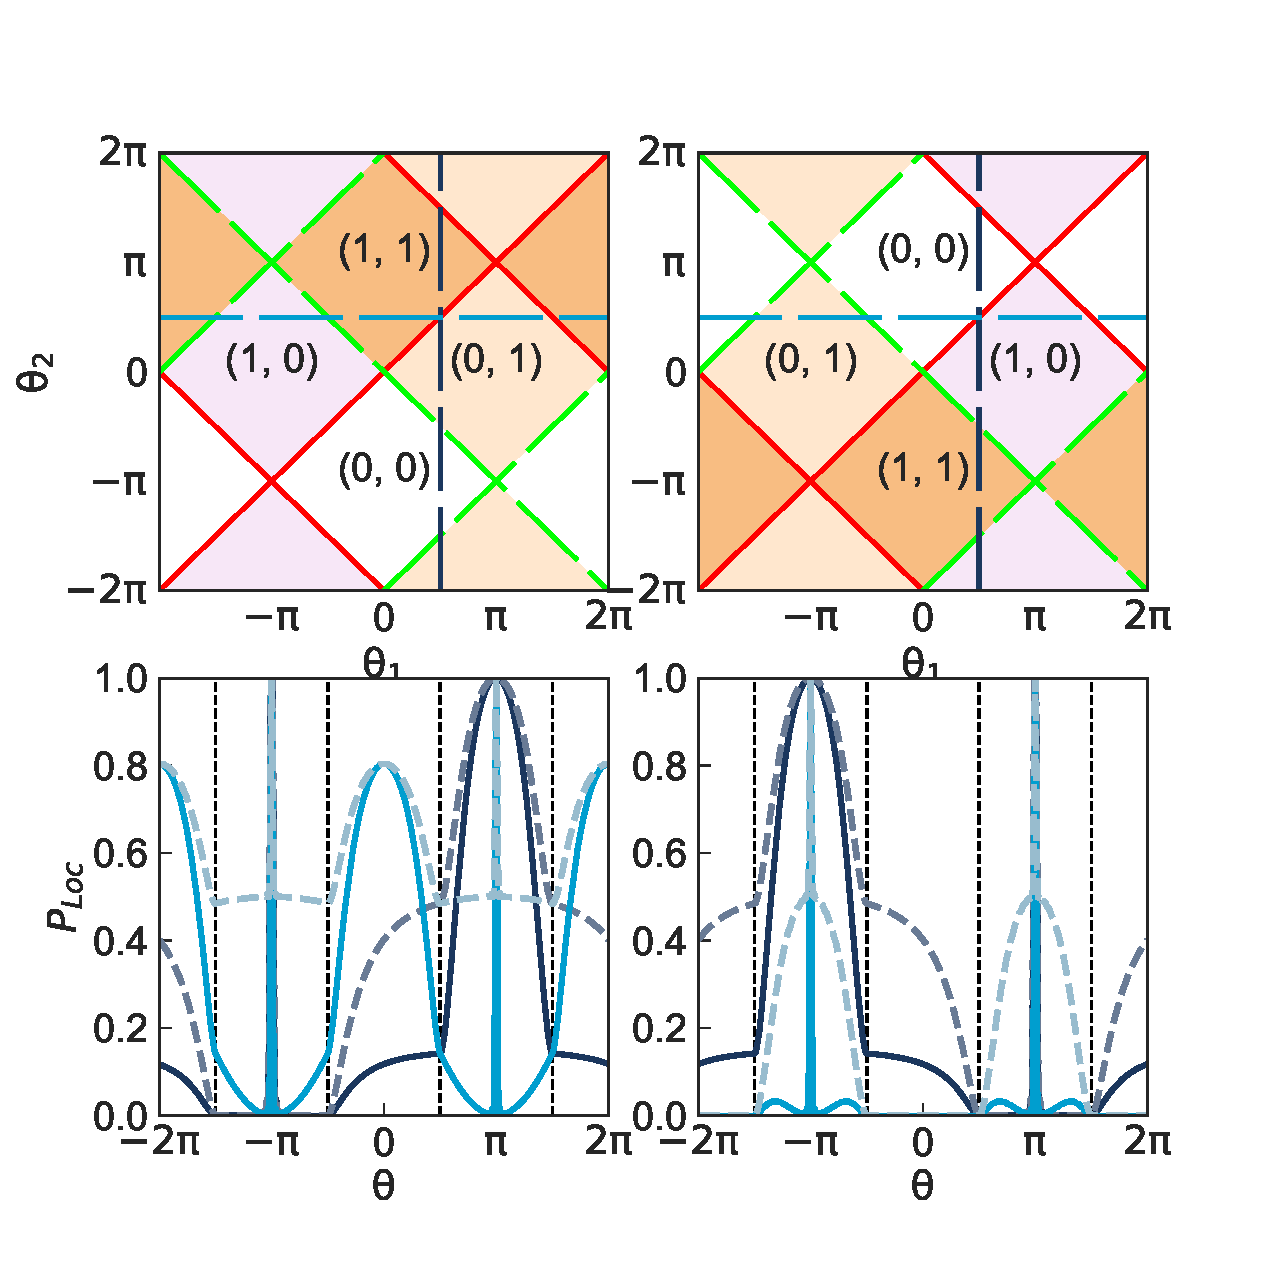
\includegraphics[width=8.5cm]{Figure/fig_3}\caption{\label{fig:3} The phase diagram of SSQW with boundary and simulatd
bound state dynamics under different parameters. (a) Phase diagram
of $\phi=0,\pi$ (left and right diagrams). The vacuum $(0,0)$ is
defined by \textquotedblleft cut link'' operation $C_{-1,0}$, which
corresponds to the region: $\theta_{2}=-\pi,\pi$ for $\phi=0,\pi$
respectively. In the phase diagram, the dashed green lines mean gap
close at $E=0$ and the soild red lines mean gap close at $E=\pi$.
By testing the parity of how many times the gap close when starting
from vacuum to another region, we know the relative topological invariant
$(\nu_{0},\nu_{\pi})$. The whole diagram is divided into four different
phases. b. simulation results after 50 steps with $\phi=0,\pi$ respectively.
The initial state is prepared onto $\left|0\right\rangle \otimes\left|\downarrow\right\rangle $.
Apperance of bound states are represented by $P_{\text{Loc}}$. The
cyan and blue curves correspond to scan over $\theta_{1}=\pi/2$ and
$\theta_{2}=\pi/2$ dashed line in a, dash lines and soild lines correspond
to two time frames introduced in Eq. \ref{eq:1} and \ref{eq:2} respectively.
Sharp boundary between different regions could be obversed from (b)
for the number of $E=0,\pi$ bound states changing. The sharpness
will also appear inside one phase, for example: the red star in $(0,1)$,
purple stars in $(1,0)$ and orange square in $(0,0)$. $E=\pi/2$
eigen-state contributes to this sharpness as explained in the main
tex.}
\end{figure}
\begin{figure}
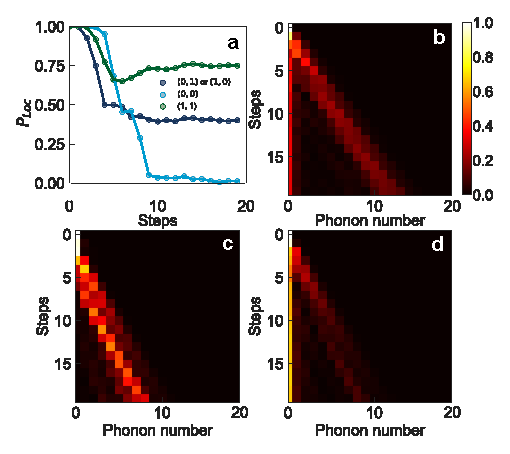
\includegraphics[width=8.5cm]{Figure/fig_4}\caption{\label{fig:4} Existence of bound state in different regions. We study
point in different topology: $(0,1):(0,\pi/2)$, $(0,0):(-3\pi/4,\pi/2)$,
$(1,1):(3\pi/4,\pi/2)$. The particle is prepared onto $\left|0\right\rangle \otimes\left|\downarrow\right\rangle $.
a. is localized possibility $P_{\text{Loc}}$ verse steps, we can
observe that $P_{\text{Loc}}$ decay to near zero after about 15 steps
when coin in the trivial phase. b $(0,1)$, c $(0,0)$, d $(1,1)$
shows $P_{\text{Loc}}$ verse steps and phonon numbers. Clear bound
state could be found at the boundary when coin in the non-trivial
phase. The brightness shows $P_{\text{Loc}}$.}
\end{figure}


\section{DYNAMICS OF BOUND STATE\label{sec:5}}

In the Sec. \eqref{sec:4}, we have verified the existence of bound
states when interfering with non-trivial bulk. In this section we
study the dynamics of bound state under time-varying bulk parameters,
both quenching and slow but non-adiabatic process. Notice that under
these process, the unitary dynamcis will not change system's topological
invariant \citep{caio2015quantum,d2015dynamical}. Instead of preparing
the system onto ground state as suggested in \citep{xu2018measuringd},
here steady-state wave function first build in one phase, which character
as $P_{\text{Loc}}$. The idea of time-dependent coin operation have
been mentioned in \citep{PhysRevA.73.062304,PhysRevLett.104.050502},
while neither dealing with bound state. Here we show how bound states
(steady-state) response to different dynamical process (further with
disorder). \textcolor{red}{We also study how changing time-frame and
breaking symmetry effects bound state -> Maybe put this into sup.
inf.} 

\emph{1. Dynamics between neighbor region}
\begin{figure}
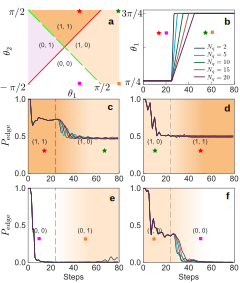
\includegraphics[width=8.5cm]{Figure/fig_5}\caption{\label{fig:5} Dynamical evolution between neighbor topological phases.
The particle is prepared onto $\left|0\right\rangle \otimes\left|\downarrow\right\rangle $.$\theta_{1}$is
time-varying while $\theta_{2}=\pi/2$ or $-\pi/2$ is fixed. a. shows
phase diagram and parameter points used. b. shows $\theta(t)$ under
different dynamical process (from $\theta_{1}^{i}$ to $\theta_{1}^{f}$).
The second row gives $P_{\text{Loc}}$verse time when evolving beetween
red star ($\pi/4,\pi/2$) and green star ($3\pi/4,\pi/2$). The result
shows that the bound state will be preserved between $(1,0)$ and
$(1,1)$. The third row studies the evolution between pink square
($5\pi/4,-\pi/2$) and orange square ($\pi/4,-\pi/2$). The result
shows that the bound state will be destroyed between $(1,0)$ and
$(0,0)$. The results above have nothing to do with the velocity of
the evolution.}
\end{figure}
Here we study the condition when across the phase boundary once. The
time-dependent coin operation under slow but non-adiabatic process
(the quench process mentioned in Sec. \ref{sec:2}) has the form:

\begin{equation}
\theta_{1}(t)=\begin{cases}
\theta_{1}^{i} & t\leq t_{0}-\tau\\
\frac{\theta_{1}^{i}+\theta_{1}^{f}}{2}+\frac{\theta_{1}^{f}-\theta_{1}^{i}}{2}\tanh(\frac{t-t_{0}}{\xi}) & t_{0}-\tau<t\leq t_{0}+\tau\\
\theta_{1}^{f} & t_{0}+\tau<t
\end{cases},
\end{equation}
where $\xi$ determine the speed of evolution between two phases.
The evolution tend to be the quench process with small $\xi$; and
to be the adiabatic evolution with large $\xi$. First $t_{0}-\tau$
steps for buliding steady-state with $\theta_{1}^{i}$. Final steps
after $t_{0}+\tau$ for buliding steady-state with $\theta_{1}^{f}$.
We still character our system with $P_{\text{Loc}}$. In Fig. \ref{fig:5},
we simulate dynamics between neighbor regions. $t_{0}$ is 40 steps
and $\tau$ is 20 steps here. In second row of Fig. \ref{fig:5},
we fix $\theta_{2}=\pi/2$, first study the situation with the neighbor
regions. We evolve $\theta_{1}$ from $\pi/4$ to $3\pi/4$, which
correspond to transfer from $(1,1)$ to ($1,0)$ (red star to green
star) and the inverse process. So we can study how bound states evolve
to another non-trivial phase. We can easily observe from the simulation
result that bound state exists after transferring to another non-trivial
phase regardless of evolution velocity (similar between $(0,1)$ and
$(1,1)$). \textcolor{red}{This could be understood by existence of
two eigen-states in $(1,1)$, then one of the eigen-state has the
same eigen-energy ($0$ or $\pi$) in neighbor phase ($(1,0)$ or
$(0,1)$)->not sure if the reason is sufficient here.}

Then we study $\theta_{2}=-\pi/2$, transfer $\theta_{1}$ from $\pi/4$
to $3\pi/4$, which correspond to transfer from $(0,0)$ to $(0,1)$
(pink square to orange square) and the inverse process. Here we study
if bound state will be built (destroyed) from trivial (non-trivial)
to non-trivial (trivial) phase. The results are in third row of Fig.
\ref{fig:5}.The particle evolves from the trivial phase to the non-trivial
phase, we can know that the bound state will not be built. Inversely,
the bound state first build in the non-trivial phase; after evolving
to the trivial phase, the bound state disappears. The conclusion in
this situation: the bound state will not build between neighbor non-trivial
and trivial phase (similar between $(0,1)$ and $(0,0)$). \textcolor{red}{for
($\nu_{0},\nu_{\pi}$) will not change under Unitary evolution->not
sure if I should say this one.}

\emph{2. Dynamics between non-neighbor regions}
\begin{figure}
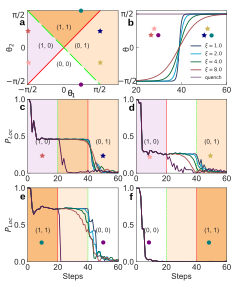
\includegraphics[width=8.5cm]{Figure/fig_6}\caption{\label{fig:6} Dynamical evolution between non-neighbor topological
phases. The particle is prepared onto $|0\rangle\otimes|\downarrow\rangle$.
The second row corresponds to the evolution between $(0,1)$ and $(1,0)$,
two paths are selected, one fixes $\theta_{2}=\pi/4$ acrossing $(1,1)$
and another fixes $\theta_{2}=-\pi/4$ acrossing the regions $(0,0)$.
The third row studies the evolution between $(1,1)$ and $(0,0)$,
which corresponds to cyan circle $(\pi/4,\pi/2)$ and purple circle
$(\pi/4,-\pi/2)$. The result shows that the bound state will be destroyed
between non-neighbor topological phase.}
\end{figure}
Here we study the condition when the evolution across phase boundary
twice. In this condition, two phases are not adjacent. We set fixed
$\theta_{1}=\pi/4$, then transfer $\theta_{2}$ from $\pi/2$ to
$-\pi/2$, which correspond to transfer from $(1,1)$ to $(0,0)$
(cyan circle to purple circle) and the inverse process. Fig. \ref{fig:6}
shows that the bound state will not be built when evolving between
$(1,1)$ and $(0,0)$, quench or slow non-adiabatic process. Similar
condition when evolving between $(1,0)$ and $(0,1)$. We set $\theta_{2}=\pi/4$
or $-\pi/4$ to be fixed and transfer between $\theta_{1}=-\pi/2$
and $\pi/2$. Two different path, one crosses the $(1,1)$ and another
across $(0,0)$, the result both no bound state could be built or
preserved.
\begin{figure}
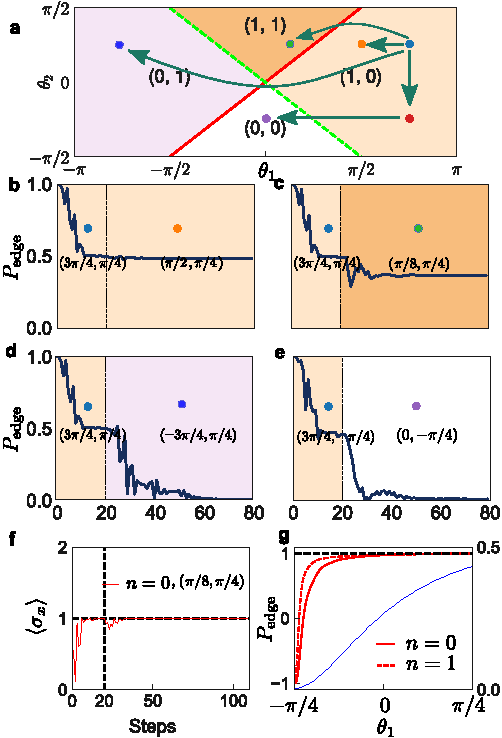
\includegraphics[width=8.5cm]{Figure/fig_7}\caption{\label{fig:7} Particular case of dynamical evolution between $(1,0)$
and $(0,1)$. The particle is prepared onto $\left|0\right\rangle \otimes\left|\downarrow\right\rangle $.
a,c,e studies the effect of evolution velocity. First 10 steps are
for building steady-state and another 50 steps for transfering the
particle to another phase under different velocity. Final 20 steps
to obtain the steady-state in the final region. $\text{\ensuremath{\theta_{1}}}$
transfers from $\pi$ to $-\pi$, in c $\theta_{2}$ is set to be
$\pi/4$ and in e is $0$. The different colors in c,d correspond
to the different velocities in a. We can observe that faster the evolution
is, larger $P_{\text{Loc}}$is. b,d,f studies the result with disorder.
b shows the sketch map of $\theta_{1}$ with disorder. $\xi$ is set
to be 10 (slow but non-adabatic conditions), bound state rarely exist
after the evolution in this condition. However, adding random disorder
to the rotation angle enhance the possibility of residue at the boundary
and stablize the bound state (reduce the oscillation patterns in the
former plot), which is similar to the non-trivial Hall responds in
Ref. \citep{hu2016dynamical}. The plot is the average of 50 random
sampling of $\delta$. From d,f, we observe that larger disorder strength
is, more the bound state is preserved.}
\end{figure}
In the former results, it seems that the results are not associated
with the evolution velocity. However, there is an exception: when
evolving between two solitons in $(1,0)$ and $(0,1)$ (as mentioned
in Sec. \ref{sec:4}, red and purple stars in Fig. \ref{fig:3}a).
\textcolor{red}{->For here two solitons have the same quasi-energy
$\pi/2$.} $P_{\text{Loc}}$ after evolution will be affected by the
evolution velocity (in former part, we show that no bound state remains
between $(1,0)$ and $(0,1)$). In Fig. \eqref{fig:7}c, $\theta_{2}=\pi/4$,
the bound state seems to have the pattern of oscillation, which can
be explained by crossing the third region $(1,1)$ during the evolution
comparing to Fig. \eqref{fig:7}e, where $\theta_{2}=0$ will not
cross a third region. $\xi=10$ is an example of nearly no bound state
is preserved. However, inducing additional disorder (defined as random
error $\theta_{1}\in[\theta-\delta,\theta+\delta]$) can help ``store''
the bound, even more stable. The strength of different disorders ($\delta$)
is shown in Fig. \eqref{fig:7}d,f, which is simulated by the average
of 50 results. As the increment of disorder strength $\delta$, $P_{\text{Loc}}$
also becomes larger. The conclusion of this special situation is that
when transferring between the solitons between $(0,1)$ and $(1,0)$,
the bound state will remain with disorder.

\section{CONCLUSION\label{sec:6}}

In this paper, we discuss the proposal to realize QW in phonon space
with carefully designed laser sequence. The boundary condition will
determine parameters region for the vacuum. Bound state will appear
under the non-trivial phase without the need of spatial-dependent
coin operation. By this convenience, the system can be used to study
the Unitary evolution of the bound state under different dynamical
processes. The behaviors of bound state will not be influenced by
the velocity when evolution between neighbor regions, two eigen-states
region and vacuum. The bound will only preserve between single eigen-state
regions and two eigen-states region. The result will be determined
by velocity when considering the evolution between two solitons. The
bound state will remain more when the evolution is more close to quench
dynamics. When introducing disorder, slow non-adiabatic dynamics bound
state also appear as increasing of disorder strength. We give reasonable
explanation for the conclusion above. See more details in Sup. \ref{sec:C}
fewer steps result for real experiment; Sup. \ref{sec:D} the potential
to study high dimension QW in our proposal; Sup. \ref{sec:E} change
time frames and symmetry during evolution.

\appendix

\section{Simple semi-infinite QW\label{sec:A}}

To understand the character of the bound state, we consider a simple
semi-infinite QW as the form of $U_{x}=S_{x}R(\theta)$ ($x=0,1,2,\cdots$)
, where $S_{x}$ is site-dependent

\begin{eqnarray}
S_{\text{0 }} & =\left|1\right\rangle \left\langle 0\right|\otimes\left|\uparrow\right\rangle \left\langle \uparrow\right|+e^{i\phi}\left|0\right\rangle \left\langle 0\right|\otimes\left|\uparrow\right\rangle \left\langle \downarrow\right| & ,\nonumber \\
S_{x>0} & =\sum_{i}\left|n-1\right\rangle \left\langle n\right|\otimes\left|\downarrow\right\rangle \left\langle \downarrow\right|+\left|n+1\right\rangle \left\langle n\right|\otimes\left|\uparrow\right\rangle \left\langle \uparrow\right|\label{eq:sup_1}
\end{eqnarray}
and the coin operator $R(\theta)$ homogeneous. There may be an additional
phase $\phi$ accumulated at site $0$. It is easy to test that $\phi=0$
or $\pi$ according to the requirement of the particle hole symmetry
(PHS). The bulk of the QW shows non-trivial winding thus it is a topological
non-trivial phase. When it interferes with the vacuum, the bound state
will appear at the boundary ($x=0$) and the energy gap will only
close at $k=0(\pi)$ with the eigen-enenergy with $0(\pi)$. The wave
function can be solved analytically ($U_{x}\left|\psi\right\rangle =e^{-iE_{b}}\left|\psi\right\rangle $)
\citep{Kitagawa2012} in this situation, for example:

\begin{eqnarray}
\left|\psi^{E=0}(i)\right\rangle  & =\frac{1}{\mathcal{N}}(-1)^{i}e^{-i/\lambda}\otimes\left(\begin{array}{c}
1-\sqrt{2}\\
1
\end{array}\right)
\end{eqnarray}
for $\theta=\pi/2$, $\phi=0$, where $\lambda=-\frac{1}{\log(\sqrt{2}-1)}$
is the localization parameter and $\mathcal{N}$ is the normalization
parameter. It is clear that there exist an exponent decay bound state
which is the eigen-state of system with eigen-energy $E=0$ in Fig.
\ref{fig:sup_1}.The particle is initially prepared on $|0\rangle\otimes|\downarrow\rangle$.
After 50 steps, a exponent decay state appears at the boundary. The
fitting localization parameter is close to $\lambda$. The bound state
will not be the exactly same state as the eigen-state solved, because
we do not prepare the particle onto the eigen-state and there will
have possibility of leaking to the bulk. We could also take this model
into our ``cut link'' discussion in the main text: the bulk SSQW
with parameter $\theta_{1}=\pi/2$ and $\theta_{2}=0$, and the boundary
condition $\phi=0$. With setting $\theta_{2}=0$, which corresponds
to a horizontal line in Fig. \ref{fig:3}a right phase diagram, crossing
two regions in the phase diagram: $0\leq\theta_{1}\leq2\pi$, $E=0$;
and when $-2\pi\leq\theta_{1}\leq0$, $E=\pi$. Same results of eigen-energy
could also be derivated from the analytical solution above.
\begin{figure}
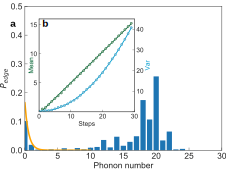
\includegraphics[width=8cm]{Figure/sup_1}\caption{\label{fig:sup_1}The simulation result with $\theta=\pi/2$ (or $\theta_{1}=\pi/2,\theta_{2}=0$
). The histogram shows the possibility distribution after 50 steps
and the orange line is the analytical solution of eigen-state. Two
subplots are the mean and variance of QW verse steps. QW with boundary
still represents acceleration of the random walk which shows the quadratic
increment of deviation.}
\end{figure}


\section{Sign of bound state\label{sec:B}}

In Fig. \eqref{fig:sup_2}, the signs of bound state is shown. Wave
fuction in $(0,1)$ with a single $E=\pi$ bound is predicted to appear
a minus signs after each steps, while in $(1,0)$ with a single $E=0$
bound state will not. After several steps building up steady-state,
the signs at $\left|0\right\rangle \otimes\left|\downarrow\right\rangle ,\left|0\right\rangle \otimes\left|\uparrow\right\rangle $
also become stable. In $(1,0)$, the signs of ($\left|\downarrow\right\rangle ,\left|\uparrow\right\rangle $)
are always $(-+)$ however in $(0,1)$ the signs will change between
$(--)$ and $(++),$ which agrees the discussion above. So different
single bound state could be distinguish. What's more, as interference
patterns of the region with two boundary will appear and no boundary
state at the vacuum phase.
\begin{figure}
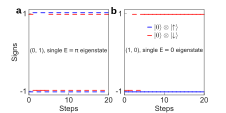
\includegraphics[width=8cm]{Figure/sup_2}\caption{\label{fig:sup_2} Signs of bound state in different regions under
SSQW. The first parameters ($\pi/2,\pi/4$) in $(0,1)$ region, corresponds
to a single $E=\pi$ eigen-state and the second parameter (-$\pi/2,\pi/4$)
in $(1,0)$ region, corresponds to a single $E=0$ eigen-state. The
initial state is prepared onto $\left|0\right\rangle \otimes\left|\downarrow\right\rangle $.
The red line in the plot shows the signs of $\left|\uparrow\right\rangle $
and the blue one shows $\left|\downarrow\right\rangle $ when setting
initial state as the criterion. It could be seen in the plot: after
several steps to build up steady state at boundary, each steps in
$(0,1)$ will change the sign of wavefunction distribution at the
boundary and walk in $(1,0)$ will not change. It could help to distinguish
$E=0$ and $E=\pi$ eigen-state.}
\end{figure}


\section{Real Experiment Time-steps\label{sec:C}}

In the discussion above, all the time-step numbers are set to be large
enough to explain the physics behind. Here we use the as little as
possible to create feasible experiment conditions. First of all, when
considering observing bound state, it could be known from Fig. \ref{fig:4}:
10 steps (or less) is enough for some parameters (for example, blue
curves) to build and observe steady bound state in the experiment.
In Fig. \ref{fig:5}, we also know that 10 steps are enough for distinguishing
between different sign (eigen-energy) of the steady bound state. In
Fig. \ref{fig:sup_3}, we simulate the result after 10 steps with
the same parameters as Fig. \ref{fig:2}. Basically, boundary between
two adjacent phases could be observed while sharpness inside one phase
($E=\pi/2$ eigen-state) could not be seen. The boundary will be more
clear when increasing the time-steps.

Second, we consider dynamics between different phase. It's easy to
understand that it will cost more steps for you need to build steady-state
in one region first then build steady-state in another phase. As in
Fig. \ref{fig:7} , quench and slow but non-adiabatic transition between
two phase give similar results. It's expected to be 10 steps or less
to build steps then quenching to another phase, evolving for another
10 steps for steady. Then the results in Fig. \ref{fig:sup_3} for
non-adiabatic with disordering, process between two phase needs to
be considered. In , total 20 steps for quenching between different
phases (($\pi/4,\pi/2$) for $(1,1)$, ($\pi/4,-\pi/2$) for $(0,1)$
and ($3\pi/4,\pi/2$) for $(1,0)$; ($-\pi/2,\pi/4$) for $(0,1)$,
($\pi/2,\pi/4$) for $(1,0)$). Similar results as mentioned former
could be observed (only the bound state of blue curve remains). In
b total 26 steps are constituted by 7 steps for steady-state in the
first phase then 12 steps non-adiabatic switching parameters to another
phase with different disorder strength and final 7 steps for steady-state
in another phase. Disorder enhanced $P_{\text{Loc}}$ is also shown
in this plot.
\begin{figure}
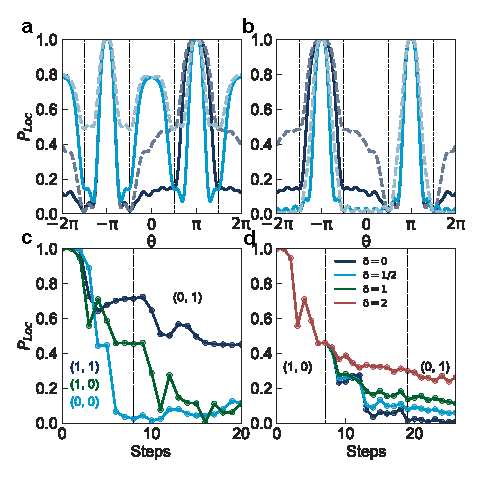
\includegraphics[width=8.6cm]{Figure/sup_3}\caption{\label{fig:sup_3} Simulation result of localization possibility after
10 steps verse different SSQW setting. The parameters are same as
Fig. \ref{fig:2}b (50 steps). a. is the plot for $\varphi=0$ and
fix one of $\theta_{1,2}$ and scan over another while b. is the plot
for $\varphi=\pi$. Simulation of dynamics with fewer steps. In c,
the initial state $\left|0\right\rangle \otimes\left|\downarrow\right\rangle $
first builds steady-state in different phase (8 steps) than quenching
(at the dashed line) to another phase for steady (12 steps). In d,
the initial state first builds steady-state in $(0,1)$ (7 steps)
then non-adiabatic transferring to ($1,0$) (6 steps), finally evolve
in $(1,0)$ (7 steps) for steady. The parameters used are same as
Fig. \ref{fig:7}.}
\end{figure}


\section{High dimensional QW\label{sec:D}}

Two dimensional QW suggested in Ref. \citep{PhysRevA.82.033429,chen2018observation,yan2019strongly,sajid2019creating,li2020two},
which could be associated with non-trivial Chern numbers and more
complex Floquet band structure. This idea could also be realized based
on our proposal. Single step with two coin operations and two walk
operations:

\begin{eqnarray}
U=S_{y}R(\theta_{2})S_{x}R(\theta_{1}),
\end{eqnarray}
where $S_{x}=\sum_{x,y}\left|x+1,y\right\rangle \left\langle x,y\right|\otimes\left|\uparrow\right\rangle \left\langle \uparrow\right|+\left|x-1,y\right\rangle \left\langle x,y\right|\otimes\left|\downarrow\right\rangle \left\langle \downarrow\right|$
and $S_{y}=\sum_{x,y}\left|x,y+1\right\rangle \left\langle x,y\right|\otimes\left|\uparrow\right\rangle \left\langle \uparrow\right|+\left|x,y-1\right\rangle \left\langle x,y\right|\otimes\left|\downarrow\right\rangle \left\langle \downarrow\right|$,
$x,y$ are independent freedoms here. $R(\theta)$ also means rotation
of the spin around y axis by angle $\theta$ here. Based on this proposal,
CS bound state can exist at the interface of Floquet insulators even
whose Chern numbers vanish, which is the unique phenomena in Periodically
driven systems \citep{Kitagawa2012,chen2018observation}. In our proposal,
two dimensions of the particle propagation are encoded onto two motional
modes of a single trapped ion: for example, the axis mode and radial
mode with cooling and resolved frequency $\omega_{z},\omega_{r}$.
What's more, Raman beams are needed in both axis and radial direction.
Based on the former 1D SSQW proposal and set $\theta_{2}=0$, $S_{x,y}R(\theta)$
can be realized with suitable Raman beams detuning of motional modes.
Of course, this 2D model has two reflecting boundary for $x,y\geq0$.
Based on this idea, arbitrary dimensional quantum walk can be realized.
More motional modes will enlarge the motional space in the high dimensional
QW with the ability of resolved sideband transition. And this high
dimensional quantum walk (more than 2D) can not be reached in the
system which walk state is encoded on position or path.

\section{Dynamics under different time frame and symmetry\label{sec:E}}

Here we study the condition which ($\theta_{1},\theta_{2}$) does
not change while quenching to another time-frame or suddenly inducing
operation to break the symmetry. In first plot of Fig. \ref{fig:sup_4},
we study the dynamics of the bound state when suddenly quenching to
another time frame: 1) change order of $\theta_{1},\theta_{2}$: $U(\theta_{2},\theta_{1})$
2) change to the first time frame preserve CS: $U_{1}(\theta_{1},\theta_{2})$
3) change to to the second time frame preserve CS: $U_{2}(\theta_{1},\theta_{2})$
(Eq. \eqref{eq:2}). And then focus on break PHS in second plot of
Fig. \ref{fig:sup_4}, which can be easily break with the coin operation
mentioned in Eq. \eqref{eq:6}. CS can also be broken with four steps
quantum walk suggested in \citep{asboth2013bulk}. We can consider
two methods to break PHS: 1) $U_{\text{break1}}=S_{+}R\left(\theta_{1},\chi\right)S_{-}R\left(\theta_{2}\right)$
2) $U_{\text{break2}}=S_{+}R\left(\theta_{1},\chi\right)S_{-}R\left(\theta_{2},\chi\right)$
($R\left(\theta\right)=\sum_{i}|i\rangle\langle i|\otimes\mathrm{e}^{-\mathrm{i}\sigma_{y}\theta/2-\mathrm{i}\chi\sigma_{z}}$).
When setting $\theta_{1}=\pi/4$, $\theta_{2}=\pi/2$. First 20 steps
SSQW is used to build steady-state, then suddenly quenching to another
time-frame or break the symmetries. The result shows the the time-frame
$U(\theta_{1},\theta_{2})$ and $U_{1}(\theta_{1},\theta_{2})$ are
very close with only slightly different effects on the stability of
bound state. The second plot shows the behavior of bound state when
inducing $\sigma_{z}$ terms in the coin operations. Blue, orange
curves shows the single $\sigma_{z}$ terms and green, red curves
shows inducing $\sigma_{z}$ terms in both coin operations. It's natural
to find that the smaller $\chi$ is, the less bound state will be
affected. After changing time-frame and breaking symmetry, the bound
state will reduce but still exist.
\begin{figure}
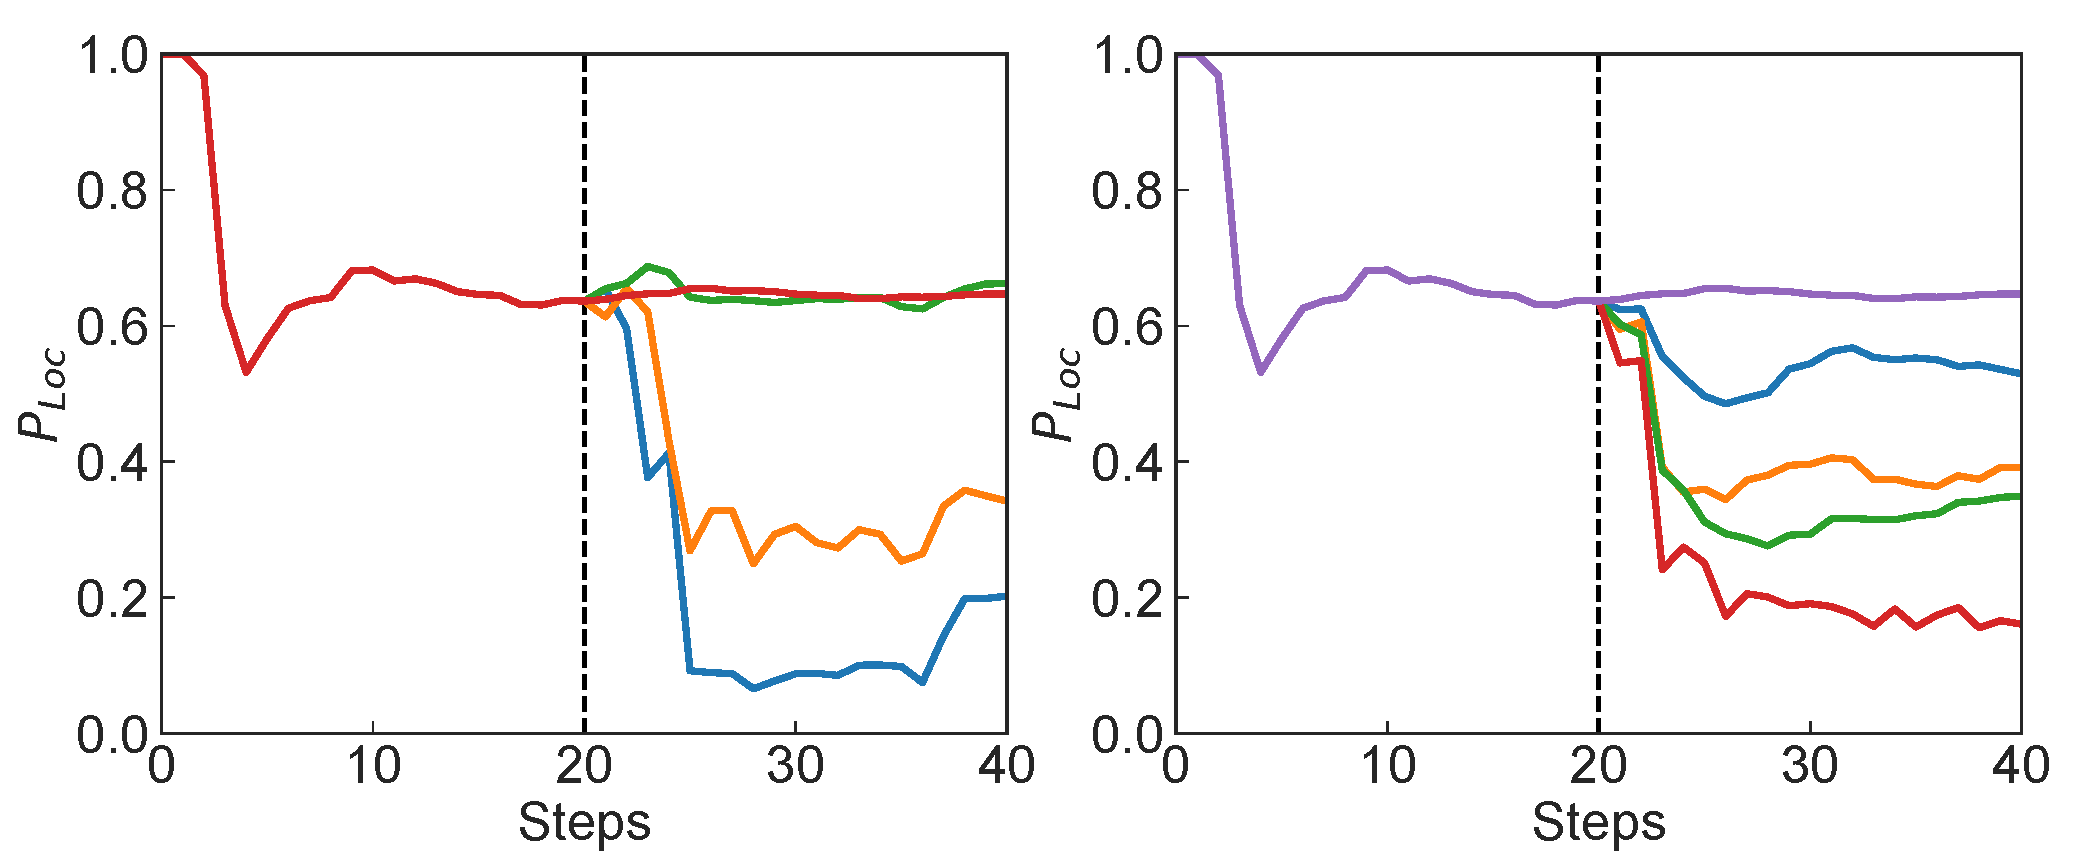
\includegraphics[scale=0.25]{Figure/sup_4}\caption{\label{fig:sup_4}Dynamics under different time-frames and symmetries.
First 20 steps is used to built steady-state, then in first plot quench
to another time-frame, in the second plot quenchs to another QW break
PHS. In the first plot, red one correponds to $U(\theta_{1},\theta_{2})=S_{-}C(\theta_{2})S_{+}C(\theta_{1})$,
the green one correponds to $U_{1}(\theta_{1},\theta_{2})$, the orange
one correponds to $U_{2}(\theta_{1},\theta_{2})$ which preserve CS
as mentioned above and the blue one correponds to $U(\theta_{2},\theta_{1})$.
In the second plot, purple one orreponds to $U(\theta_{1},\theta_{2})$,
green ($\chi=\pi/4$) and red ($\chi=\pi/2$) one correponds to the
first methods to break PHS, blue ($\chi=\pi/4$) and orange ($\chi=\pi/2$)
one correponds to the second methods to break PHS.}
\end{figure}


\appendix
\bibliographystyle{apsrev4-1}
\phantomsection\addcontentsline{toc}{section}{\refname}\nocite{*}
\bibliography{qw}

\end{document}
